\chapter{Области на Скот}
\index{област на Скот}

В тази глава ще разгледаме понятията, които са ни нужни за дефинирането на понятието денотационна семантика на една програма.

\section{Частични наредби}
\index{частична наредба}

Бинарната релация $\sqsubseteq$ върху множеството $A$ се нарича {\bf частична наредба}, ако тя е:
\marginpar{На англ. \emph{partial order}}
\begin{itemize}
\item 
  рефлексивна, т.е. $(\forall a \in A)[a \sqsubseteq a]$;
\item
  транзитивна, т.е. $(\forall a,b,c \in A)[a \sqsubseteq b\ \&\ b \sqsubseteq c \implies a \sqsubseteq c]$;
\item
  антисиметрична, т.е. $(\forall a,b \in A)[a \sqsubseteq b\ \&\ b \sqsubseteq a  \implies a = b]$.
\end{itemize}

Една такава двойка $(A, \sqsubseteq)$ се нарича частично наредено множество.

\begin{example}
  Да означим 
  \[\Partial{\Nat}{\Nat} \dff \{f:\Nat\to\Nat \mid f\text{ е частична функция}\}.\]
  Дефинираме и релацията {\bf включване } между две частични функции по следния начин:
  \begin{align*}
    f \subseteq g \dfff (\forall x\in \Nat)[& f(x)\text{ не е деф.}\ \vee\\
                                            & (f(x)\text{ е деф.}\ \&\ g(x)\text{ е деф.}\ \&\ f(x) = g(x))].
  \end{align*}
  Да дефинираме също {\bf графиката} на частичната функция $f$ като
  \[\Graph{f} \dff \{\pair{x,y} \mid f(x) = y\}.\]
  Тогава лесно се съобразява, че 
  \[f \subseteq g \iff \Graph{f} \subseteq \Graph{g}.\]
  Съобразете, че двойката $(\Partial{\Nat}{\Nat}, \subseteq)$ е частично наредено множество.
\end{example}

Казваме, че $a_0$ е {\bf най-малък елемент} на частично нареденото множество $(A, \sqsubseteq)$,
ако $(\forall a \in A)[a_0 \sqsubseteq a]$. Ако такъв елемент съществува, то той е единствен,
защото релацията $\sqsubseteq$ е антисиметрична.

{\bf Неподвижна точка} на $f:A \to A$ е елемент $a \in A$, такъв че $f(a) = a$.

За по-кратко, монотонно-растящите редици от елементи на $A$,
\[a_0 \sqsubseteq a_1 \sqsubseteq \cdots \sqsubseteq a_n \sqsubseteq \cdots,\]
ще наричаме (растящи) {\bf вериги}. 

Един елемент $b$ е {\bf горна граница} на веригата $\chain{a}{n}$, ако 
$(\forall n)[a_n \sqsubseteq b]$.
Един елемент $b$ е {\bf точна горна граница} на веригата $\chain{a}{n}$, ако са изпълнени свойствата:
\begin{itemize}
\item 
  $(\forall n)[a_n \sqsubseteq b]$, т.е. $b$ е горна граница;
\item
  за всяка друга горна граница $c$ е изпълнено, че $b \sqsubseteq c$, т.е.
  $b$ е най-малкият елемент измежду всички горни граници на веригата $\chain{a}{n}$.
\end{itemize}
Не всяка верига притежава точна горна граница.
Обикновено точната горна граница на вергата $\chain{a}{n}$ ще бележим като $\bigsqcup_n a_n$.

Наредена тройка от вида $\A = (A, \sqsubseteq, \bot)$ се нарича {\bf област на Скот}, ако:
\index{област на Скот}
\marginpar{На англ. {\em Scott domain}}
\begin{itemize}
\item
  $\sqsubseteq$ е бинарна релация върху $A$, която задава частична наредба.
\item
  Всяка растяща верига $\chain{a}{n}$ в $A$ притежава точна горна граница $\bigsqcup_n a_n$.
\item
  $\bot \in A$ е най-малкият елемент на $A$;
\end{itemize}

\marginpar{В Хаскел $\bot$ се означава като \vv{undefined}. Повече за денотационна семантика в Хаскел може да прочетете \href{https://en.wikibooks.org/wiki/Haskell/Denotational_semantics}{тук}}

\begin{example}
  \Stefan{Друго означение вместо $\F_n$ ?}
  Тройката
  \[\F_n \dff (\ \Partial{\Nat^n}{\Nat},\subseteq, \emptyset^{(n)}\ )\] е област на Скот, където:
  \begin{itemize}
  \item
    С $\Partial{\Nat^n}{\Nat}$ означаваме всички частични функции от $\Nat^n$ в $\Nat$.
  \item
     релацията ,,включване'' между функции е дефинирана по следния начин:
     \[f\subseteq g\ \dffff\ (\forall \bar{x})(\forall y)[ f(\bar{x}) \simeq y \implies  g(\bar{x}) \simeq y].\]
   \item
     $\emptyset^{(n)}$ е функцията с празна дефиниционна област, т.е.
     \[(\forall \bar{x} \in \Nat^n)[\neg !\emptyset^{(n)}(\bar{x})].\]
  \end{itemize}
\end{example}

\begin{example}
  Да разгледаме няколко примера, които вече сме срещали.
  \begin{itemize}
  \item
    $(\Ps(\Nat),\subseteq,\emptyset)$ е област на Скот.
  \item
    $(\Nat, \leq, 0)$ не е е област на Скот.
  \item
    $(\Nat\cup\{\infty\}, \leq, 0)$ е също област на Скот, където $0 \leq 1 \leq \cdots \leq \infty$.
  \item
    $(\{0,1\}^\star, \preceq, \varepsilon)$ не е област на Скот, където $\preceq$ е релацията префикс на две думи.
    % Може да образувате безкрайна растяща верига от думи, но тяхната точна горна граница ще бъде безкрайна дума.
  \end{itemize}
\end{example}

\begin{example}
  Да разгледаме множеството 
  \[Bin^\infty = \{\sigma \mid \sigma :\{0,1,2,\dots,n-1\} \to \{0,1\}\ \&\ n \in \Nat\} \cup 
  \{f \mid f:\Nat \to \{0,1\}\}\]
  съставено от всички крайни и безкрайни двоични низове.
  \begin{itemize}
  \item
    Да разгледаме релацията
    \[\sigma \preceq \tau \iff \abs{\sigma} \leq \abs{\tau}\ \&\ (\forall i < |\sigma|)[\sigma(i) = \tau(i)],\]
    $\sigma$ е префикс на $\tau$.    
  \item
    Да означим с $\varepsilon$ единствения двоичен низ с дължина $0$.
  \end{itemize}
  Тогава $Bin^\infty = (Bin^\infty,\preceq,\varepsilon)$ е област на Скот.
\end{example}

Още тук да се дефинира $\Mapping{\Nat_\bot}{\Nat_\bot}$ и да се види, че образува област на Скот.

%%% Local Variables:
%%% mode: latex
%%% TeX-master: "../sep"
%%% End:


\section{Конструкции}

Ще разгледаме няколко конструкции, с които ще видим как можем да строим по-сложни области на Скот.

\subsection{Плоска област на Скот}

\Stefan{По принцип плоската област на Скот се дефинира върху друга област на Скот}

Да фиксираме едно произволно непразно множество $A$ и един елемент $\bot \not \in A$.
Да означим $A_\bot = A \cup \{\bot\}$ и да разгледаме следната бинарна релация $\sqsubseteq$ върху $A_\bot$:
\[a \sqsubseteq b\ \iff\ a = \bot\ \vee\ a = b.\]
Лесно се съобразява, че $\sqsubseteq$ задава {\em частична наредба} върху $A_\bot$:
\marginpar{От деф. на $\sqsubseteq$ следва, че $\bot$ е най-малкият елемент}
\begin{itemize}
\item 
  {\em рефлексивност}: $a \sqsubseteq a$ за всяка $a \in A_\bot$;
\item
  {\em транзитивност}: $a \sqsubseteq b\ \&\ b \sqsubseteq c \implies a\sqsubseteq c$ за всеки $a,b,c \in A_\bot$;
\item
  {\em антисиметричност}: $a \sqsubseteq b\ \&\ b\sqsubseteq a \implies a = b$ за всеки $a,b \in A_\bot$.
\end{itemize}

Наредбата $(A_\bot, \sqsubseteq)$ ще наричаме {\bf плоска наредба}. Тя ще играе важна роля в нашите разглеждания.
\marginpar{$\bot$ се нарича {\em bottom} елемент}
Например, често ще разглеждаме плоската наредба $(\Nat_\bot, \sqsubseteq)$.

\begin{example}
  Плоската наредба $(\Nat_\bot, \sqsubseteq)$ може да се изобрази по следния начин.
  \begin{framed}
  \begin{figure}[H]
    \label{fig:flat-nat-1}
    \centering
    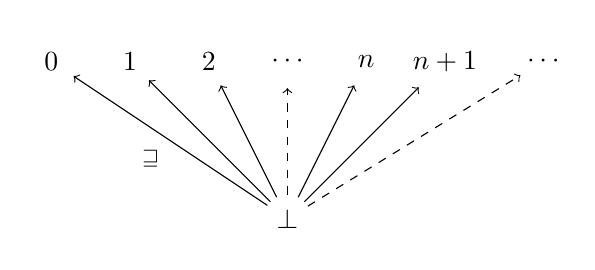
\begin{tikzpicture}[shorten >=1pt,->]
      \tikzstyle{vertex}=[circle,minimum size=17pt,inner sep=0pt]
      
      \node[vertex] (bot) at (3,0) {$\bot$};
      \node[vertex] (0) at (0,2) {$0$};
      \node[vertex] (1) at (1,2) {$1$};
      \node[vertex] (2) at (2,2) {$2$};
      \node[vertex] (dots) at (3,2) {$\cdots$};
      \node[vertex] (n) at (4,2) {$n$};
      \node[vertex] (n1) at (5,2) {$n+1$};
      \node[vertex] (ddots) at (6.25,2) {$\cdots$};
      
      \draw (bot) -- node[below left]{$\scriptstyle{\sqsupseteq}$} (0);
      \draw (bot) -- (1);
      \draw (bot) -- (2);
      \draw[dashed] (bot) -- (dots);
      \draw (bot) -- (n);
      \draw (bot) -- (n1);
      \draw[dashed] (bot) -- (ddots);
    \end{tikzpicture}    
    \caption{Графично представяне на $\sqsubseteq$ върху $\Nat_\bot$}
  \end{figure}
  \end{framed}
\end{example}

\begin{prop}
  \index{област на Скот!плоска}
  Нека $A$ е произволно множество и нека елементът $\bot \not \in A$.
  \marginpar{На англ. {\em flat domain}}
  Определяме наредената тройка $\A_\bot = (A_\bot, \sqsubseteq, \bot)$ като:
  \begin{itemize}
  \item 
    $A_\bot = A\cup\{\bot\}$;
  \item
    $\sqsubseteq$ задава {\em плоската наредба} върху $A_\bot$.
  \end{itemize}
  Тогава $\A_\bot$ е област на Скот, която ще наричаме {\bf плоска област на Скот} за множеството $A$.
\end{prop}


%%% Local Variables:
%%% mode: latex
%%% TeX-master: "../sep-notes"
%%% End:


\subsection{Крайно произведение}
\label{subsect:domains:product}
\index{област на Скот!крайно произведение}
\marginpar{\cite[стр. 125]{winskel}}

Нека $\A$ и $\B$ са области на Скот.
Тогава $\A \times \B \df (A \times B,\sqsubseteq,\bot)$, където
\begin{itemize}
\item
  $A \times B = \{\pair{a,b} \mid a \in A\ \&\ b \in B\}$;
\item
  $\pair{a,b} \sqsubseteq \pair{a',b'} \iff a \sqsubseteq^\A a'\ \&\ b \sqsubseteq^\B b'$;
\item
  $\bot = \pair{\bot^\A,\bot^\B}$.
\end{itemize}

\begin{framed}
  \begin{proposition}
    \label{pr:cartesian}
    Ако $\A$ и $\B$ са области на Скот, то $\A \times \B$ е област на Скот.
  \end{proposition}  
\end{framed}
\begin{hint}
  Лесно се съобразява, че $\sqsubseteq$ е частична наредба и че $\bot$ е най-малкият елемент.
  Да разгледаме една верига $\{\pair{a_i,b_i}\}^\infty_{i=1}$ в $\A \times \B$.
  Лесно се вижда, че
  \[\bigsqcup_i\pair{a_i,b_i} = \pair{\bigsqcup_ia_i,\bigsqcup_ib_i}.\]
  \begin{itemize}
  \item
    За произволен елемент $\pair{a_i,b_i}$ от веригата е ясно, че $a_i \sqsubseteq^\A \bigsqcup_ia_i$ и $b_i \sqsubseteq^\B \bigsqcup_i b_i$.
    Следователно, $\pair{\bigsqcup_ia_i,\bigsqcup_ib_i}$ е горна граница на веригата.
  \item
    Нека $\pair{c,d}$ е горна граница на веригата, т.е. за всяко $i$,
    $a_i \sqsubseteq^\A c$ и $b_i \sqsubseteq^\B d$.
    Но тогава $c$ е горна граница на веригата $\chain{a}{i}$ и следователно $\bigsqcup_ia_i \sqsubseteq^\A c$.
    Също така, $d$ е горна граница на веригата $\chain{b}{i}$ и следователно $\bigsqcup_i b_i \sqsubseteq^\B d$.
    Заключаваме, че $\pair{\bigsqcup_ia_i,\bigsqcup_ib_i} \sqsubseteq \pair{c,d}$, т.е. $\pair{\bigsqcup_ia_i,\bigsqcup_ib_i}$
    е точна горна граница на веригата.
  \end{itemize}
\end{hint}

Нека $\A_1,\dots,\A_n$, $n \geq 2$, са области на Скот. Дефинираме 
$\prod^n_{i=1}\A_i = (A, \sqsubseteq, \bot)$ по следния начин:
\begin{itemize}
\item
  Ако $n = 2$, то $\prod^2_{i=1} \A_i \df \A_1 \times \A_2$.
\item
  Ако $n > 2$, то $\prod^n_{i=1} \A_i \df (\prod^{n-1}_{i=1}\A_i) \times \A_n$.
\end{itemize}

Използвайки \Prop{cartesian}, лесно се съобразява следното твърдение.
\begin{proposition}
  Ако $\A_1,\dots,\A_n$, $n \geq 2$, са области на Скот, то $\prod^n_{i=1}\A_i$ е област на Скот.
\end{proposition}

\begin{framed}
  \begin{figure}[H]
    \centering
    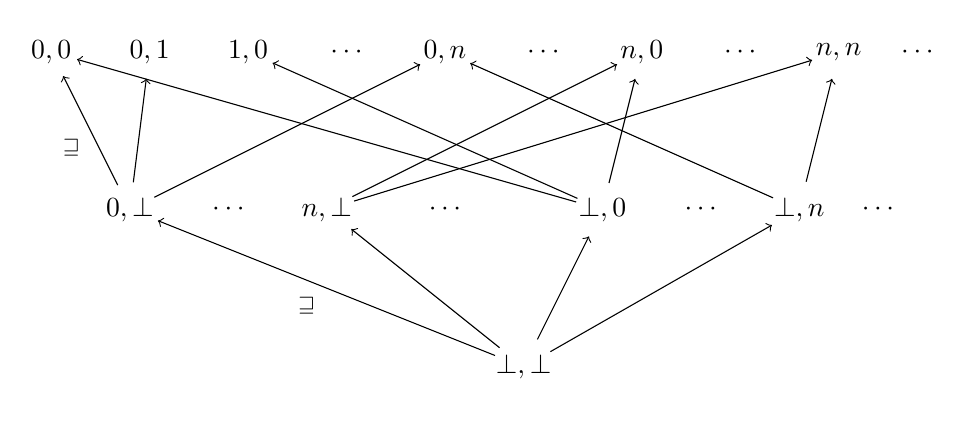
\begin{tikzpicture}[shorten >=1pt,->]
      \tikzstyle{vertex}=[circle,minimum size=17pt,inner sep=0pt]
      
      \node[vertex] (bot) at (5,-1) {$\pair{\bot,\bot}$};
      
      \node[vertex] (0b) at (0,1) {$\pair{0,\bot}$};
      \node[vertex] (db) at (1.25,1) {$\cdots$};
      \node[vertex] (nb) at (2.5,1) {$\pair{n,\bot}$};
      \node[vertex] (ddb) at (4,1) {$\cdots$};
      
      \node[vertex] (b0) at (6,1) {$\pair{\bot,0}$};
      \node[vertex] (bd) at (7.25,1) {$\cdots$};
      \node[vertex] (bn) at (8.5,1) {$\pair{\bot,n}$};
      \node[vertex] (bdd) at (9.5,1) {$\cdots$};
      
      \node[vertex] (00) at (-1,3) {$\pair{0,0}$};
      \node[vertex] (01) at (0.25,3) {$\pair{0,1}$};
      \node[vertex] (10) at (1.5,3) {$\pair{1,0}$};
      \node[vertex] (ddd) at (2.75,3) {$\cdots$};
      \node[vertex] (0n) at (4,3) {$\pair{0,n}$};
      \node[vertex] (dddd) at (5.25,3) {$\cdots$};
      \node[vertex] (n0) at (6.5,3) {$\pair{n,0}$};
      \node[vertex] (ddddd) at (7.75,3) {$\cdots$};
      \node[vertex] (nn) at (9,3) {$\pair{n,n}$};
      \node[vertex] (dddddd) at (10,3) {$\cdots$};

      \draw (bot) -- node[below left]{$\scriptstyle{\sqsupseteq}$} (0b);
      \draw (bot) -- (nb);
      \draw (bot) -- (b0);
      \draw (bot) -- (bn);

      \draw (0b) -- node[below left]{$\scriptstyle{\sqsupseteq}$} (00);
      \draw (0b) -- (01);
      \draw (0b) -- (0n);

      \draw (b0) -- (00);
      \draw (b0) -- (10);
      \draw (b0) -- (n0);
      \draw (nb) -- (n0);
      
      \draw (nb) -- (nn);
      \draw (bn) -- (0n);
      \draw (bn) -- (nn);

    \end{tikzpicture}    
    \caption{Графично представяне на част от $\sqsubseteq$ върху $\Nat^2_\bot$}
    \label{fig:flat-nat-2}
  \end{figure}
\end{framed}

Вижда се от \Fig{flat-nat-2}, че всяка верига в $\Nat^2_\bot$ има дължина най-много $3$.
Лесно се съобразява, че всяка верига в $\Nat^k_\bot$ има дължина най-много $k+1$.
Свойството, че всяка верига в $\Nat^k_\bot$ има само краен брой различни члена
ще се окаже важно по-нататък. Сега ще въведем понятие, което описва това свойство в произволна област на Скот.
\marginpar{ $\Nat^k_\bot = \underbrace{\Nat_\bot \times \cdots \times\Nat_\bot}_{k}$}

Нека $\A$ е област на Скот и да разгледаме една верига $\chain{a}{n}$ в $\A$.
Ще казваме, че $\chain{a}{n}$ се {\bf стабилизира}, ако съществува индекс $n_0$, за който
\[(\forall n \geq n_0)[a_{n_0} = a_{n}],\]
т.е.
\[a_0 \sqsubseteq a_1 \sqsubseteq a_2 \sqsubseteq \cdots \sqsubseteq a_{n_0} = a_{n_0+1} = a_{n_0+2} = \cdots\]
От казаното по-горе следва, че всяка растяща верига в $\Nat^k_\bot$ се стабилизира.

\marginpar{Едни от основните области на Скот, които ще разглеждаме при дефинирането на денотационната семантика ще бъдат $\Nat_\bot$ и $\Nat^k_\bot$.}


%%% Local Variables:
%%% mode: latex
%%% TeX-master: "../sep"
%%% End:


\section{Изображения в области на Скот}

\index{област на Скот!изображения}
Нека $\A_i = (A_i,\sqsubseteq_i,\bot_i)$, за $i = 1,2$, са области на Скот.
Ще въведем няколко основни вида изображения между $\A_1$ и $\A_2$, 
които ще използваме често. След това ще разгледаме някои свойства на тези изображения
и ще видим каква е връзката между тях.
\begin{itemize}
\item
  Всяка тотална функция от вида $f:A_1 \to A_2$ ще наричаме изображение между областите на Скот $\A_1$ и $\A_2$
  и ще записваме $f:\A_1 \to \A_2$.
  Да въведем означението 
  \[\Mapping{\A_1}{\A_2} \dff \{f \mid f:\A_1 \to \A_2\}.\]
\item
  Да въведем следната релация между изображенията $f,g:\A_1 \to \A_2$:
  \[f \sqsubseteq g \dfff (\forall a \in \A_1)[f(a) \sqsubseteq_2 g(a)].\]
\item
  Да дефинираме изображението $\bm{\bot}:\A_1 \to \A_2$ като
  \[(\forall a \in \A_1)[\bm{\bot}(a) = \bot_2].\]
\end{itemize}

  \begin{haskellcode}
ghci> let bottom _ = undefined
  \end{haskellcode}

\begin{framed}
  \begin{thm}
    \label{th:all-mappings-is-domain}
    Наредената тройка $(\Mapping{\A_1}{\A_2}, \sqsubseteq, \bm{\bot})$ е област на Скот.
  \end{thm}  
\end{framed}
\begin{proof}
  Нетривиалната част в доказателството е да проверим, че всяка верига $(f_i)^{\infty}_{i=0}$ в $\Mapping{\A_1}{\A_2}$
  притежава точна горна граница.
  \marginpar{За по-кратко пишем $\bar{a}$ вместо $a_1,\dots,a_n$}
  Да разгледаме изображението $h:\A_1 \to \A_2$, където:
  \begin{equation}
    \label{eq:9}
    h(a) \dff \bigsqcup \{f_i(a) \mid i \in \Nat\}.
  \end{equation}
  Ще докажем, че $h$ е тази точна горна граница.
  \begin{itemize}
  \item
    \marginpar{Това задължително трябва да се провери,
      защото например множеството $\{\bot, 0, 3\}$ няма точна горна граница относно плоската наредба в $\Nat_\bot$}
    Първо, трябва да се убедим, че дефиницията на $h$ е ,,смислена'', т.е. $h$ е тотална функция.
    Трябва да докажем, че за всяко $a\in \A_1$,
    \[\bigsqcup\{f_i(a) \mid i \in \Nat\}\] съществува.
    Да фиксираме произволен елемент $a \in \A_1$.
    Получаваме следната верига в $\A_2$:
    \[f_0(a) \sqsubseteq f_1(a) \sqsubseteq f_2(a) \sqsubseteq \cdots \]
    Понеже $\A_2$ е област на Скот, то тази верига притежава точна горна граница в $\A_2$,
    която означачаваме като $\bigsqcup\{f_i(a) \mid i \in \Nat\}$.
    Това означава, че $h(a)$ е тотална функция.
  \item
    Дотук имаме, че $h \in \Mapping{\A_1}{\A_2}$.
    Лесно се съобразява, че $h$ е горна граница на веригата $\chain{f}{i}$, защото за всяки елемент $a \in \A_1$
    и произволен индекс $i$,
    \[f_i(a) \sqsubseteq \bigsqcup\{f_i(a) | i \in \Nat\} \dff h(a).\]
  \item
    Сега остава да проверим, че $h$ е точна горна граница, т.е. $h$ е най-малката измежду всички горни граници на 
    веригата $\chain{f}{i}$.
    Нека $g$ е друга горна граница на $\chain{f}{i}$. Това означава, че за всеки индекс $i$,
    $f_i \sqsubseteq g$. Следователно, за фиксирано $a \in \A_1$,
    $g(a)$ е горна граница за веригата $(f_i(a))^{\infty}_{i=0}$.
    Тогава е ясно, че за разглеждания елемент $a$,
    \[h(a) \dff \bigsqcup\{f_i(a) \mid i\in\Nat\} \sqsubseteq g(a).\]
    Понеже елементът $a$ е прозиволен, получаваме, че $h \sqsubseteq g$.
  \item
    Доказахме, че $h$ е горна граница и че $h$ е най-малката измежду всички горни граници.
    Заключваме, че $h$ е {\em точна горна граница} на веригата $\chain{f}{i}$.
    \marginpar{Получаваме, че \[(\bigsqcup_if_i)(a) = \bigsqcup_i\{f_i(a)\}.\]}
    С други думи,
    \[h = \bigsqcup_i f_i.\]
  \end{itemize}
\end{proof}

\begin{cor}
  $(\Mapping{\Nat^n_\bot}{\Nat_\bot},\sqsubseteq, \bm{\bot}^{(n)})$ е област на Скот,
  където $\bm{\bot}^{(n)}(\bar{a}) = \bot$, за всяко $\bar{a} \in \Nat^n_\bot$.
\end{cor}


%%% Local Variables:
%%% mode: latex
%%% TeX-master: "../sep"
%%% End:


\subsection{Монотонни изображения}

\index{изображение!монотонно}
Да разгледаме областите на Скот $\A_1 = (A_1, \sqsubseteq_1, \bot_1)$ и $\A_2 =(A_2, \sqsubseteq_2, \bot_2)$.
Едно изображение $f:\A_1\to \A_2$ се нарича {\bf монотонно}, ако
\[(\forall a,a'\in\A_1)[a \sqsubseteq_1 a' \implies f(a) \sqsubseteq_2 f(a')].\]
Да въведем означението
\[\Mon{\A_1}{\A_2} \dff \{f: \A_1 \to \A_2 \mid f\text{ е монотонно изобр.}\}.\]


\Stefan{Да се обясни каква е интерпретацията на монотонните изображения в нашия частен случай и защо на практика това е най-естествения клас от изображения, с който ще работим}

\begin{framed}
  \begin{thm}
    \label{th:monotone-is-domain}
    $(\Mon{\A_1}{\A_2},\ \sqsubseteq, \bot)$ е област на Скот.
  \end{thm}  
\end{framed}
\begin{hint}
  Да фиксираме една верига $\chain{f}{i}$ в $\Mon{\A_1}{\A_2}$. Трябва да докажем, че тази верига притежава точна горна граница,
  която е монотонно изображение.
  Да разгледаме същото изображение $h:\A_1 \to \A_2$ както в доказателството на \Th{all-mappings-is-domain}, като
  \[h(a) \dff \bigsqcup_i \{f_i(a) \mid i \in \Nat\}.\]
  Оттам знаем, че $h$ е точна горна граница на веригата. 
  Остава да докажем, че $h \in \Mon{\A_1}{\A_2}$.
  Нека $a \sqsubseteq b$. Тогава, понеже $f_k$ са монотонни изображения,
  \[(\forall k)[f_k(a) \sqsubseteq f_k(b) \sqsubseteq \bigsqcup_i \{f_i(b) \mid i \in \Nat\} \dff h(b)].\]
  Това означава, че $h(b)$ е горна граница за веригата $(f_i(a))^{\infty}_{i=0}$.
  Заключаваме, че 
  \begin{align*}
    h(a) & \dff \bigsqcup \{f_i(a) \mid i \in \Nat\}\\
         & \sqsubseteq \bigsqcup \{f_i(b) \mid i \in \Nat\} \dff h(b).    
  \end{align*}
\end{hint}

\begin{cor}
  \label{cr:flat-monotone-is-domain}
  $(\Mon{\Nat^n_\bot}{\Nat_\bot},\ \sqsubseteq, \Omega^{(n)})$ е област на Скот.
\end{cor}


%%% Local Variables:
%%% mode: latex
%%% TeX-master: "../sep-notes"
%%% End:


\subsection{Непрекъснати изображения}
\index{изображение!непрекъснато}

\marginpar{На англ. {\em continuous}}
Едно изображение $f:\A_1\to \A_2$ се нарича {\bf непрекъснато}, ако
при всеки избор на верига $\chain{a}{n}$ в $\A_1$, то имаме равенството
\marginpar{Понеже $\A_1$ е област на Скот знаем, че $\bigsqcup_i a_i \in \A_1$}
\marginpar{$\bigsqcup_if(a_i) \dff \bigsqcup\{f(a_i) \mid i \in \Nat\}$}
\[f(\bigsqcup_i a_i) = \bigsqcup_i f(a_i).\]
С други думи, 
$f(\bigsqcup_i a_i)$ е точната горна граница в $\A_2$ на множеството 
\[\{f(a_n) \mid n \in \Nat\}.\]
Да означим
\[\Cont{\A_1}{\A_2} \dff \{f: \A_1 \to \A_2 \mid f\text{ е непр. изобр.}\}.\]


\begin{framed}
  \begin{prop}
    \label{pr:continuous-is-monotone}
    За произволни области на Скот $\A_1$ и $\A_2$, всяко непрекъснато изображение $f:\A_1 \to \A_2$ е монотонно, т.е.
    \[\Cont{\A_1}{\A_2}\ \subseteq\ \Mon{\A_1}{\A_2}.\]
  \end{prop}
\end{framed}
\begin{proof}
  Нека $f \in \Cont{\A_1}{\A_2}$.
  Да вземем два произволни елемента в $\A_1$, за които $a \sqsubseteq_1 b$.
  Ще докажем, че $f(a) \sqsubseteq_2 f(b)$.
  
  Да разгледаме веригата $\chain{a}{i}$ в $\A_1$, където:
  \[\underbrace{a_0}_{a} \sqsubseteq \underbrace{a_1}_{b} = \underbrace{a_2}_{b} = \underbrace{a_3}_{b} = \cdots\]

  Ясно е, че 
  \[\bigsqcup_i\{a_i \mid i \in \Nat\} = \bigsqcup\{a,b\} = b.\]
  Тогава от непрекъснатостта на $f$ имаме, че
  \begin{align*}
    f(a) & = f(a_0) & \comment{\text{защото }a_0 \dff a}\\
    & \sqsubseteq_2 \bigsqcup\{f(a_i) \mid i \in \Nat\} & \comment{\text{защото }f(a_0) \in \{f(a_i) \mid i\in\Nat\}}\\
    & = f(\bigsqcup_i a_i) & \comment{\text{защото $f$ е непр.}}\\
    & = f(\bigsqcup\{a,b,b,b,\dots\}) & \comment{\text{от избора на веригата }\chain{a}{i}}\\
    & = f(b) & \comment{\text{защото }a \sqsubseteq_1 b}.
  \end{align*}
  Така получихме, че за произволни $a,b\in\A_1$, 
  \[a \sqsubseteq_1 b \implies f(a) \sqsubseteq_2 f(b).\]
\end{proof}

% \begin{cor}
%   \label{cr:continuous-is-monotone}
%   $\Cont{\Nat^n_\bot}{\Nat_\bot} \subseteq \Mon{\Nat^n_\bot}{\Nat_\bot}$.
% \end{cor}

\begin{prop}
  Съществува област на Скот $\A$, за която
  \[\Cont{\A}{\A} \subsetneqq \Mon{\A}{\A}.\]
\end{prop}
\begin{hint}
  Нека $A = \{a_n \mid n \in \Nat\} \cup \{a_\omega, b_0\}$.
  Да разгледаме областта на Скот $\A = (A, \sqsubseteq, a_0)$, където 
  наредбата между елементите е следната:
  \[a_0 \sqsubseteq a_1 \sqsubseteq \cdots \sqsubseteq a_n \sqsubseteq \cdots \sqsubseteq a_\omega \sqsubseteq b_0. \]
  Нека $f(a_n) = a_{n+1}$ и $f(a_{\omega}) = b_0$.
  Очевидно е, че $f$ е монотонно изображение.
  Лесно се вижда, че $f$ не е непрекъснато изображение, 
  защото $f(\bigsqcup_n a_n) = f(a_\omega) = b_0$,
  но 
  \[\bigsqcup_n f(a_n) = \bigsqcup_n a_{n+1} = a_\omega.\]
\end{hint}

Сега да видим един важен за нас случай, при който имаме и обратното включване.

\begin{framed}
  \begin{prop}
    \label{pr:stab-continuous}
    Ако всяка верига в $\A_1$ се {\em стабилизира}, то
    \[\Mon{\A_1}{\A_2} \subseteq \Cont{\A_1}{\A_2}.\]
  \end{prop}  
\end{framed}
\begin{hint}
  Да разгледаме една верига $\chain{a}{i}$ и $f \in \Mon{\A_1}{\A_2}$.
  Ще докажем, че \[f(\bigsqcup_i a_i) = \bigsqcup_i f(a_i).\]

  \begin{enumerate}[(1)]
  \item 
    Ясно е, че за всяко монотонно изображение $f$,
    понеже $a_i \sqsubseteq \bigsqcup_i a_i$, то $f(a_i) \sqsubseteq f(\bigsqcup_i a_i)$.
    Това означава, че $f(\bigsqcup_i a_i)$ е горна граница на веригата $(f(a_i))^\infty_{i=0}$
    и следователно $\bigsqcup_i f(a_i) \sqsubseteq f(\bigsqcup_i a_i)$.
  \item
    За другата посока ще използваме свойството, че веригата $\chain{a}{i}$ се стабилизира.
    Нека $n_0$ е индекс, такъв че $(\forall k \geq n_0)[a_k = a_{n_0}]$.
    Това означава, че $\bigsqcup_i a_i = a_{n_0}$.
    Тогава $f(\bigsqcup_i a_i) = f(a_{n_0}) \sqsubseteq \bigsqcup_i f(a_i)$.    
  \end{enumerate}
  
  От $(1)$ и $(2)$ следва, че $f(\bigsqcup_i a_i) = \bigsqcup_i f(a_i)$.
\end{hint}

Понеже всяка верига в $\Nat^n_\bot$ се {\em стабилизира}, то
получаваме следното важно следствие.
\begin{framed}
\begin{cor}
  \label{cr:monotone-is-continuous}
  $\Mon{\Nat^n_\bot}{\Nat_\bot} = \Cont{\Nat^n_\bot}{\Nat_\bot}$.
\end{cor}  
\end{framed}

От доказателството на (1) за \Prop{stab-continuous} можем да извлечем следното свойство,
което ще ни бъде полезно по-нататък.
\begin{prop}
  \label{pr:monotone-chain}
  За всяко изображение $f \in \Mon{\A}{\B}$ и всяка верига $\chain{a}{i}$, е изпълнено, че
  \[\bigsqcup_i f(a_i) \sqsubseteq f(\bigsqcup_i a_i).\]
\end{prop}

Понеже от \Cor{flat-monotone-is-domain} имаме, че монотонните изображения образуват област на Скот, 
то директно получаваме следната важна теорема.

\begin{framed}
\begin{thm}
  \label{th:continuous-is-domain}
  $(\Cont{\Nat^n_\bot}{\Nat_\bot},\ \sqsubseteq,\ \Omega^{(n)})$ е област на Скот.
\end{thm}  
\end{framed}
% \begin{proof}
%   От \Cor{monotone-is-continuous} имаме, че 
%   \[\Mon{\Nat^n_\bot}{\Nat_\bot} = \Cont{\Nat^n_\bot}{\Nat_\bot}.\]
%   От \Cor{flat-monotone-is-domain} имаме, че 
%   \[(\Mon{\Nat^n_\bot}{\Nat_\bot}, \sqsubseteq, \Omega^{(n)})\]
%   е област на Скот. 
%   Оттук директно получаваме, че 
%   \[(\Cont{\Nat^n_\bot}{\Nat_\bot}, \sqsubseteq, \Omega^{(n)})\] е област на Скот.
% \end{proof}


% \begin{prop}
%   \label{pr:composition}
%   \index{изображения!композиция}
%   Ако $f \in \Cont{\A}{B}$ и $g \in \Cont{\B}{\C}$, то $g \circ f \in \Cont{\A}{\C}$,
%   където \[(g\circ f)(a) \dff g(f(a)).\]
% \end{prop}
% \begin{hint}
%   Нека $\chain{a}{i}$ е верига в $\A$.
%   Да обърнем внимание, че понеже $f \in \Cont{\A}{\B}$,
%   то $f$ е монотонно изображение и тогава $(f(a_i))^\infty_{i=0}$ е верига в $\B$.
%   Тогава:
%   \begin{align*}
%     (g \circ f)(\bigsqcup_i a_i) & = g(f(\bigsqcup_i a_i)) & \comment{\text{от деф.}}\\
%     & = g(\bigsqcup_i f(a_i)) & \comment{f \text{ е непр.}}\\
%     & = \bigsqcup_i g(f(a_i)) & \comment{g \text{ е непр.}}
%   \end{align*}
% \end{hint}

%%% Local Variables:
%%% mode: latex
%%% TeX-master: "../sep-notes"
%%% End:


\subsection{Точни изображения}

\marginpar{На англ. се нарича {\em strict}. ,,Стандартната'' семантика на хаскел е {\em non-strict}}
\index{изображение!точно}
Едно изображение $f:\A^n_1 \to \A_2$ се нарича {\bf точно}, ако 
\[(\forall \bar{a}\in\A^n_1)[\bot_1\in\{a_1,\dots,a_n\} \implies f(a_1,\dots,a_n) = \bot_2].\]
% Тук ще разглеждаме съвкупността от точни изображения:
% \[S_n \dff \{f: \Nat^n_\bot \to \Nat_\bot \mid f\text{ е точна}\}.\]
За произволни области на Скот $\A_1$ и $\A_2$, ще означаваме съвкупността от
точните изображения като $\Strict{\A_1}{\A_2}$.

\begin{example}
  Да разгледаме свойствата на няколко прости изображения.
  \begin{itemize}
  \item 
    Изображението $f:\Nat_\bot \to \Nat_\bot$, дефинирано като 
    \[f(x) = 42,\]
    за всяко $x \in \Nat_\bot$,
    {\bf не е точно}, защото $f(\bot) = 42$. Лесно се вижда, че $f$ е монотонно и непрекъснато изображение.
  \item
    От друга страна, изображението $g:\Nat_\bot \to \Nat_\bot$, дефинирано като 
    \[g(x) = \bot,\]
    за всяко $x \in \Nat_\bot$, {\bf е точно}, защото $g(\bot) = \bot$.
    Освен това, $g$ е монотонно и непрекъснато изображение.
  \end{itemize}
\end{example}

Видяхме, че лесно се намират монотонни изображения, които не са точни.
Сега ще разгледаме обратната посока.

\begin{proposition}
  \label{pr:strict-is-monotone}
  Всяко точно изображение $f:\Nat^n_\bot \to \Nat_\bot$ е също така и монотонно.
  С други думи, 
  \[\Strict{\Nat^n_\bot}{\Nat_\bot} \subseteq \Mon{\Nat^n_\bot}{\Nat_\bot}.\]
\end{proposition}
\begin{proof}
  Нека $f$ е точно и $\bar{a} \sqsubseteq \bar{b}$.
  Ще проверим, че 
  \[f(\bar{a}) = c \sqsubseteq d = f(\bar{b}).\]
  \begin{itemize}
  \item 
    Ако $c = \bot$, то е очевидно, че $c \sqsubseteq d$.
  \item
    Интересният случай е когато $c \neq \bot$. Тогава трябва да видим, че $c = d$.
    Понеже $f$ е точна и $c \neq \bot$, това означава, че $\bot \not\in\{a_1,\dots,a_n\}$.
    Но понеже $\sqsubseteq$ е плоска наредба, и $\bar{a} \sqsubseteq \bar{b}$, това означава, че $\bar{a} = \bar{b}$.
    Следотвателно, наистина $c = d$.
  \end{itemize}
\end{proof}

\begin{framed}
  \begin{theorem}
    \label{th:strict-is-domain}
    $(\Strict{\Nat^n_\bot}{\Nat_\bot},\ \sqsubseteq,\ \bm{\bot}^{(n)})$ е област на Скот.
  \end{theorem}
\end{framed}
\begin{hint}
  Да разгледаме веригата $\chain{f}{i}$ от елементи на $\Strict{\Nat^n_\bot}{\Nat_\bot}$.
  Трябва да докажем, че тази верига притежава точна горна граница, която също е точно изображение.
  % Понеже от \Prop{strict-is-monotone} имаме, че всяка точна функция е монотонна, то наготово от 
  От доказателството на \Th{all-mappings-is-domain} знаем, че изображението $h$ дефинирано за всяко $\bar{a} \in \Nat^n_\bot$ като
  \[h(\bar{a}) \df \bigsqcup \{f_i(\bar{a}) \mid i \in \Nat\}\]
  е точна горна граница на веригата $\chain{f}{i}$.
  Остава да проверим, че $h$ е точно изображение.
  Нека $\bar{a} \in \Nat^n_\bot$ и да приемем, че $\bot \in \{a_1,\dots,a_n\}$.
  Тогава:
  \begin{align*}
    h(\bar{a}) & = \bigsqcup \{f_i(\bar{a}) \mid i \in \Nat\} & \comment{\text{от деф. на }h}\\
               & = \bigsqcup\{\bot,\bot,\dots,\bot,\dots\} & \comment{f_i\text{ са точни}}\\
               & = \bot.
  \end{align*}
\end{hint}

\begin{example}
  \label{ex:simple-non-continuous}
  Нека сега да разгледаме $h:\Nat_\bot \to \Nat_\bot$, където 
  \begin{align*}
    h(x) = &
    \begin{cases}
      0, & \text{ако }x = \bot,\\
      1, & \text{иначе}.
    \end{cases}
  \end{align*}
  Да видим колко ,,лошо'' изображение е $h$:
  \begin{itemize}
  \item 
    $h$ не е точно, защото $h(\bot) \neq \bot$;
  \item
    $h$ не е монотонно, защото $\bot \sqsubseteq 5$, но $h(\bot) = 0 \not\sqsubseteq 1 = h(5)$;
  \item
    $h$ не е непрекъснато, защото $\Cont{\Nat_\bot}{\Nat_\bot} = \Mon{\Nat_\bot}{\Nat_\bot}$.
  \end{itemize}
  Нека да видим, че хаскел не позволява такива ,,лоши'' функции:

  \begin{haskellcode}
ghci> let h(x) = if x == undefined then 0 else 1
ghci> h(5)
*** Exception: Prelude.undefined
ghci> h(undefined)
*** Exception: Prelude.undefined
  \end{haskellcode}
\end{example}

\begin{example}
  \label{ex:non-strict-monotone}
  Да разгледаме $f:\Nat^2_\bot \to \Nat_\bot$ дефинирано като \[f(x,y) = x.\]
  \begin{itemize}
  \item 
    $f$ не е точно, защото $f(0,\bot) = 0$.
  \item
    $f$ е монотонно, защото ако $\pair{x,y} \sqsubseteq \pair{x',y'}$, то $x \sqsubseteq x'$ и
    \[f(x,y) = x \sqsubseteq x' = f(x',y').\]
  \item
    $f$ е непрекъснато, защото от \Cor{monotone-is-continuous} знаем, че 
    $\Mon{\Nat^2_\bot}{\Nat_\bot} = \Cont{\Nat^2_\bot}{\Nat_\bot}$.
  \end{itemize}
\end{example}

Можем да обобщим всичко, което направихме дотук, със следната илюстрация на основните области на Скот, с които ще работим
в \Chapter{rec}.

\begin{framed}
    \begin{align*}
      \Strict{\Nat^n_\bot}{\Nat_\bot} & \subsetneqq \Mon{\Nat^n_\bot}{\Nat_\bot} & \comment{\text{от \Ex{non-strict-monotone} и \Prop{strict-is-monotone}}}\\
      & = \Cont{\Nat^n_\bot}{\Nat_\bot} & \comment{\text{от \Prop{continuous-is-monotone} и \Cor{monotone-is-continuous}}}\\
      & \subsetneqq \Mapping{\Nat^n_\bot}{\Nat_\bot} & \comment{\text{от \Ex{simple-non-continuous}}}.
    \end{align*}
\end{framed}

\begin{example}
  \label{ex:plus}
  Да разгледаме $f:\Nat^2_\bot \to \Nat_\bot$ дефинирана по следния начин:
  \[f(x,y) = 
  \begin{cases}
    \bot, & x = \bot\ \&\ y = \bot\\
    x, & x \neq \bot\ \&\ y = \bot\\
    y, & x = \bot\ \&\ y \neq \bot\\
    x+y, & x \neq \bot\ \&\ y \neq \bot.
  \end{cases}\]
  Изображението $f$ не е точно, защото например $f(\bot,0) \neq \bot$.
  $f$ не е монотонно изображение, защото $\pair{2,\bot} \sqsubseteq \pair{2,3}$, но $2 = f(2,\bot) \not\sqsubseteq f(2,3) = 5$.
  Също така, $f$ не е непрекъснато изображение, защото $\Mon{\Nat^2_\bot}{\Nat_\bot} = \Cont{\Nat^2_\bot}{\Nat_\bot}$.
\end{example}
% \begin{hint}
%   \begin{itemize}
%   \item 
%     $f$ не е точно изображение, защото например
%     $f(\bot,0) \neq \bot$.
%   \item
%     $f$ не е монотонно. Например,
%     \[\pair{\bot,0} \sqsubseteq \pair{1,0}\ \&\ f(\bot,0) = 0 \not\sqsubseteq 1 = f(1,0).\]    
%   \item
%     $f$ не е непрекъснато, защото $\Cont{\Nat^2_\bot}{\Nat_\bot} = \Mon{\Nat^2_\bot}{\Nat_\bot}$.
%   \end{itemize}    
% \end{hint}


% \subsection{Точни продължения}
% \index{изображение!точно продължение}

% Нека $A$ и $B$ са произволни множества, а $\A_\bot$ и $\B_\bot$ са плоските области на Скот получени съответно от $A$ и $B$.
% За еднa частична функция $f:A^n \to B$, определяме точното изображение $f^\star:\A^n_\bot \to \B_\bot$ по следния начин:
% \marginpar{$f^\star \in \Strict{\A^n_\bot}{\B_\bot}$}
% \begin{align*}
%   f^\star(\ov{a}) \dff
%   \begin{cases}
%     f(\ov{a}), & \text{ако }\bot\not\in\{a_1,\dots,a_n\}\ \&\ f(\ov{a})\text{ е деф.}\\
%     \bot, & \text{иначе}.
%   \end{cases}
% \end{align*}
% Изображението $f^\star$ се нарича {\bf точно продължение} на $f$.

% \begin{example}
%   Да разгледаме частичната функция $f:\Nat^2 \to \Nat$, дефинирана като
%   $f(x,y) = x+y$. Тогава точното продължение на $f$ е 
%   \[f^\star(x,y) = 
%   \begin{cases}
%     x+y, & x,y\in\Nat\\
%     \bot, & x = \bot \vee y = \bot.
%   \end{cases}\]
% \end{example}

% \Stefan{За какво ми е точното продължение да е непрекъснато?}
% \noindent Да дефинираме оператор $\Sigma^\star : \Partial{\Nat^n}{\Nat} \to \Strict{\Nat^n_\bot}{\Nat_\bot}$ като
% \[\Sigma^\star(f) = f^\star.\] 
% Ще наричаме $\Sigma^\star$ {\bf продължаващ} оператор, защото на всяка частична функция дава нейното точно продължение.

% \begin{framed}
%   \begin{prop}
%     $\Sigma^\star$ е непрекъснато изображение, т.е.
%     \[\Sigma^\star \in \Cont{\Partial{\Nat^n}{\Nat}}{\Strict{\Nat^n_\bot}{\Nat_\bot}}.\]
%   \end{prop}
% \end{framed}
% \begin{hint}
%   Трябва да докажем, че за произволна верига $(f_i)^{\infty}_{i=0}$ от частични функции, 
%   $\Sigma^\star(\bigcup_i f_i) = \bigsqcup_i \Sigma^\star(f_i)$.
%   \begin{itemize}
%   \item 
%     Лесно се съобразява, че ако $f \subseteq g$, то $\Sigma^\star(f) \sqsubseteq \Sigma^\star(g)$.
%     Оттук следва, че 
%     \[\bigsqcup_i \Sigma^\star(f_i) \sqsubseteq \Sigma^\star(\bigcup_i f_i).\]
%   \item
%     За другата посока,
%     Нека $\Sigma^\star(\bigcup_i f_i)(\ov{x}) = y \neq \bot$.
%     Това означава, че $\ov{x} \in \Nat^n$ и $(\bigcup_i f_i)(\ov{x}) \simeq y$.
%     Оттук следва, че съществува $i_0$, за което $f_{i_0}(\ov{x}) \simeq y$.
%     Тогава $\Sigma^\star(f_{i_0})(\ov{x}) = y$.
%     Понеже $y \neq \bot$, 
%     \[\bigsqcup_i (\Sigma^\star(f_i)(\ov{x})) = (\bigsqcup_i \Sigma^\star(f_i))(\ov{x}) = y.\]
%     Заключаваме, че $\Sigma^\star(\bigcup_i f_i)(\ov{x}) \sqsubseteq \bigsqcup_i (\Sigma^\star(f_i)(\ov{x}))$
%   \end{itemize}
% \end{hint}

% \Stefan{Това означава, че някъде трябва да се каже, че $\F_n$ е област на Скот. Някъде в тази глава трябва да е. Това може да бъде един от първите примери след дефиницията на О.С.}



%%% Local Variables:
%%% mode: latex
%%% TeX-master: "../sep"
%%% End:


\subsection{Точни ограничения}
\index{изображение!точно ограничение}

Нека фиксираме две области на Скот $\A$ и $\B$.
За едно изображение $f \in \Mapping{\A^n}{\B}$, дефинираме точното изображение $f_\star \in \Strict{\A^n}{\B}$ по следния начин:
\[f_\star(\bar{a}) =
\begin{cases}
  f(\bar{a}), & \text{ако } \bot\not\in\{a_1,\dots,a_n\}\\
  \bot, & \text{ако }\bot\in\{a_1,\dots,a_n\}.
\end{cases}\]
Ще казваме, че $f_\star$ е {\bf точно ограничение} на $f$.

\begin{framed}
  \begin{prop}
    За всяко $f \in \Mapping{\A^n}{\B}$, имаме 
    \[f_\star \sqsubseteq f.\]
  \end{prop}
\end{framed}

\begin{example}
  Точното ограничение на функцията $f$ от \Ex{plus} е
  \[f_\star(x, y) =
  \begin{cases}
    x + y, & \text{ако } x \neq \bot\ \&\ y \neq \bot\\
    \bot, & \text{иначе}
  \end{cases}
\]
\end{example}

\begin{example}
  Да видим какъв резултат връща хаскел при следните извиквания:
  
  \begin{haskellcode}
ghci> (\x -> 5) 4
5
ghci> (\x -> 5) undefined
5
  \end{haskellcode}
  
  От второто извикване се вижда, че в хаскел, анонимната функция $\lambda x.5$ е дефинирана и върху $\bot$ и връща отново $5$.
  \marginpar{$(\lambda x.5)(4) = 5$, $(\lambda x.5)(\bot) = 5$}
  Това е естествено, понеже хаскел е {\em неточен} език, т.е. една функция може да има като аргумент $\bot$
  и да връща ,,смислен'' резултат. 

  \marginpar{Повече информация за \texttt{seq} може да се намери в \cite[стр. 108]{real-world-haskell}}
  При разглеждането на семантики на езици за програмиране, ще се нуждаем от това да направим една функция {\em точна}.
  Такава възможност има и в хаскел с командата \texttt{seq}.
  
  \begin{haskellcode}
ghci> :t seq
seq :: a -> b -> b
ghci> (\x -> x `seq` 5) 4
5
ghci> (\x -> x `seq` 5) undefined
*** Exception: Prelude.undefined
ghci> :set -XBangPatterns
ghci> (\(!x) -> 5) undefined
*** Exception: Prelude.undefined
\end{haskellcode}
  
  Командата \texttt{seq} приема два аргумента. Тя работи като оценява първия аргумент, като очаква той да се оцени до ,,смислен'' резултат, т.е. нещо различно от $\bot$. След това връща втория.
  Тук първия пример се превежда като $(\lambda x. 5)_\star(4) = 5$, а втория като $(\lambda x.5)_\star(\bot) = \bot$.
\end{example}

За произволно естествено число $n$, да дефинираме изображение
\[\Sigma_\star : \Mapping{\Nat^n_\bot}{\Nat_\bot} \to \Strict{\Nat^n_\bot}{\Nat_\bot},\]
където
\[\Sigma_\star(f) = f_\star.\] 
Ще наричаме $\Sigma_\star$ {\bf ограничаващ} оператор, защото на всяка функция дава нейното точно ограничение.

\begin{framed}
\begin{prop}
  \label{pr:strict-operator}
  За всяко $n$, $\Sigma_\star$ е непрекъснат оператор, т.е.
  \[\Sigma_\star \in \Cont{\Mapping{\Nat^n_\bot}{\Nat_\bot}}{\Strict{\Nat^n_\bot}{\Nat_\bot}}.\]
\end{prop}  
\end{framed}
\begin{hint}
  Трябва да докажем, че за произволна верига $\chain{f}{i}$ от елементи на $\Mapping{\Nat^n_\bot}{\Nat_\bot}$, имаме
  \[\Sigma_\star(\bigsqcup_i f_i) = \bigsqcup_i \Sigma_\star(f_i).\]
  \begin{enumerate}[(1)]
  \item 
    Лесно се съобразява, че $\Sigma_\star$ е монотонно изображение, т.е.
    \[f \sqsubseteq g \implies \Sigma_\star(f) \sqsubseteq \Sigma_\star(g).\]
    Сега използваме \Prop{monotone-chain}, откъдето следва, че
    \[\bigsqcup_i \Sigma_\star(f_i) \sqsubseteq \Sigma_\star(\bigsqcup_i f_i).\]
  \item
    За другата посока, нека да разгледаме $\ov{a}$, за които
    \marginpar{Случаят $\Sigma_\star(\bigsqcup_i f_i)(\ov{a}) = \bot$ е тривиален.}
    \[\Sigma_\star(\bigsqcup_i f_i)(\ov{a}) = b \neq \bot.\]
    Щом $b \neq \bot$, то ако $\ov{a} = (a_1, \dots, a_n)$, със сигурност $\bot \not\in \{a_1, \dots, a_n\}$.
    Тогава директно имаме, че $(\bigsqcup_i f_i)(\ov{a}) = b \neq \bot$.
    Сега от \Problem{sup-f} получаваме, че съществува $i_0$, за което $f_{i_0}(\ov{a}) = b$.
    Ясно е, че също така $\Sigma_\star(f_{i_0})(\ov{a}) = b$ и оттук
    $(\bigsqcup_i \Sigma_\star(f_i))(\ov{a}) = b$,
    защото $\Sigma_\star(f_{i_0}) \sqsubseteq \bigsqcup_i \Sigma_\star(f_i)$.
    Заключаваме, че
    \[\Sigma_\star(\bigsqcup_i f_i) \sqsubseteq \bigsqcup_i\Sigma_\star(f_i).\]
  \end{enumerate}
\end{hint}

%%% Local Variables:
%%% mode: latex
%%% TeX-master: "../sep-notes"
%%% End:


\section{Най-малки неподвижни точки}
\index{най-малка неподвижна точка}

\begin{itemize}
\item 
  \index{неподвижна точка}
  Да фиксираме произволна област на Скот $\A = (A, \sqsubseteq, \bot)$ и да разгледаме едно изображение $f:\A\to\A$.
  Казваме, че $a \in \A$ е {\bf неподвижна точка} на $f$, ако $f(a) = a$.
\item
  \index{най-малка неподвижна точка}
  Казваме, че $a \in \A$ е {\bf най-малката неподвижна точка} на $f$, ако:
  \begin{itemize}
  \item 
    $a$ е неподвижна точка, т.е. $f(a) = a$;
  \item
    за всяко $b \in \A$ със свойството, че $f(b) = b$ имаме $a \sqsubseteq b$.
  \item
    \marginpar{least fixed point}
    Ще означаваме най-малката неподвижна точка на $f$ като $\lfp(f)$.
  \end{itemize}
\end{itemize}

\begin{framed}
\begin{thm}[Клини]
  \label{th:knaster-tarski}
  \index{Клини}
  Нека $\A$ е област на Скот.
  Всяко $f \in \Cont{\A}{\A}$ притежава най-малка неподвижна точка.
\end{thm}
\end{framed}
\begin{proof}
  \marginpar{В \cite{ditchev-soskov} се нарича теорема на Кнастер-Тарски. Според \href{https://en.wikipedia.org/wiki/Kleene_fixed-point_theorem}{уикипедия} е теорема на Клини}
  Определяме монотонно растяща редица от елементи на $\A$ по следния начин:
  \begin{align*}
    & a_0 \dff \bot & \comment = f^0(\bot)\\
    & a_{n+1} \dff f(a_n) & \comment = f^{n+1}(\bot).
  \end{align*}

  Първо ще докажем с индукция по $n$, че $\chain{a}{n}$ е верига.
  Ясно е, че $a_0 \sqsubseteq a_1$.
  Да приемем, че $a_n \sqsubseteq a_{n+1}$. Тогава, понеже всяко непрекъснато
  изображение е монотонно, то имаме, че
  \[\underbrace{f(a_n)}_{a_{n+1}} \sqsubseteq \underbrace{f(a_{n+1})}_{a_{n+2}}.\]

  Нека $a \dff \bigsqcup_i a_i$. Тогава 
  \begin{align*}
    f(a) & = f(\bigsqcup_i a_i) & \comment a \dff \bigsqcup_i a_i\\
         & = \bigsqcup_i f(a_i) & \comment f \text{ е непрекъсната}\\
         & = \bigsqcup_i a_{i+1} & \comment a_{i+1} = f(a_i)\\
         & = \bigsqcup_i a_i & \comment \text{защото }\chain{a}{i}\text{ е верига}\\
         & = a.
  \end{align*}
  Така доказахме, че $a$ е {\em неподвижна точка} на $f$.
  Остана да видим, че е най-малката неподвижна точка на $f$.

  Нека $b = f(b)$. С индукция по $n$ ще докажем, $(\forall n)[a_n \sqsubseteq b]$.
  \begin{itemize}
  \item 
    За $n = 0$ е очевидно.
  \item
    Да приемем, че $a_n \sqsubseteq b$.
    Тогава $a_{n+1} \dff f(a_n) \sqsubseteq f(b) = b$, защото $f$ е монотонно изображение.    
  \end{itemize}
  Така доказахме, че $b$ е горна граница на веригата $\chain{a}{n}$.
  Заключаваме, че $a \dff \bigsqcup_n a_n \sqsubseteq b$.
  Следователно, $a$ е {\em най-малката неподвижна точка} на $f$,
  т.е. $a = \lfp(f)$.
\end{proof}

\begin{prop}
  \label{pr:prefix-point}
  За всяко $f \in \Cont{\A}{\A}$ е изпълнено, че 
  \[(\forall a \in \Pref(f))[\lfp(f) \sqsubseteq a],\]
  където
  \index{преднеподвижна точка}
  \[\Pref(f) \dff \{a \in \A \mid f(a) \sqsubseteq a\}\]
  е множеството от всички преднеподвижни точки на $f$.
  Това означава, че $\lfp(f)$ е най-малката преднеподвижна точка на $f$.
\end{prop}
\begin{proof}
  Знаем от Теоремата на Клини, че $\lfp(f) = \bigsqcup_n f^n(\bot)$.
  Нека за улеснение $b_n \dff f^n(\bot)$.
  От доказателството на \hyperref[th:knaster-tarski]{Теоремата на Клини} знаем, че $\chain{b}{n}$ е верига.
  Ясно е също, че $\texttt{Pref}(f) \neq \emptyset$, защото $\lfp(f) \in \texttt{Pref}(f)$.
  Да фиксираме прозиволен елемент $a\in \texttt{Pref}(f)$.
  С индукция по $n$ ще докажем, че $b_n \sqsubseteq a$ за всяко $n$.
  \begin{itemize}
  \item 
    За $n = 0$ е очевидно, защото тогава $b_0 \dff \bot \sqsubseteq a$.
  \item
    Да приемем, че $b_n \sqsubseteq a$.
    Ще докажем, че $b_{n+1} \sqsubseteq a$.
    Но това е лесно.
    \begin{align*}
      b_{n+1} & = f(b_n) & \comment \text{от деф. на }b_{n+1}\\
      & \sqsubseteq f(a) & \comment b_n \sqsubseteq a\ \&\ f\text{ е мон.}\\
      & \sqsubseteq a & \comment a \in \texttt{Pref}(f).
    \end{align*}
  \end{itemize}
  Така доказахме, че за всяко $n$, $b_n \sqsubseteq a$,
  откъдето следва, че $a$ е горна граница за веригата $\chain{b}{n}$, откъдето директно получаваме, че
  \[\lfp(f) = \bigsqcup_n b_n \sqsubseteq a.\]
\end{proof}


%%% Local Variables:
%%% mode: latex
%%% TeX-master: "../sep-notes"
%%% End:


\section{Най-малко решение на система от уравнения}

\begin{problem}
  % \label{pr:cartesian-continuous}
  Нека $f \in \Cont{\A}{\B}$ и $g \in \Cont{\A}{\C}$.
  Докажете, че $h \in \Cont{\A}{\B\times\C}$, където
  \[h(a) \dff \pair{f(a),g(a)}.\]
  В такъв случай ще означаваме $h = f \times g$.
\end{problem}
\begin{proof}
  Нека $(a_i)^{\infty}_{i=0}$ е верига в $\A$. Тогава:
  \begin{align*}
    h(\bigsqcup_i a_i) & = \pair{f(\bigsqcup_i a_i), g(\bigsqcup_i a_i)} & \comment{\text{от деф.}}\\
    & = \pair{\bigsqcup_i f(a_i), \bigsqcup_i g(a_i)} & \comment{\text{$f$ и $g$ са непр.}}\\
    & = \bigsqcup_i \pair{f(a_i),g(a_i)} & \comment{\text{от \Prop{cartesian}}}\\
    & = \bigsqcup_i h(a_i) & \comment{\text{от деф.}}
  \end{align*}
\end{proof}

Обърнете внимание на следващото твърдение, защото ще го използваме често по-късно.
То представлява обобщение на предишната задача и има сходно доказателство.
% Първо да въведем следното означение за произволно области на Скот $\B_1,\dots,\B_n$,
% \[\prod^n_{i=1}\B_i \dff \B_1\times \B_2 \times \cdots \B_n,\]
% което също е област на Скот, дефинирана в {\em Раздел \ref{subsect:domains:product}}.

\begin{prop}
  \label{pr:product-continuous}
  Нека $f_i \in \Cont{\A}{\B_i}$, за $i = 1,\dots,n$.
  \marginpar{\writedown Докажете сами!}
  Тогава
  \[g \in \Cont{\A}{\prod^n_{i=1}\B_i},\]
  където
  \[g(a) \dff \pair{f_1(a),f_2(a),\dots,f_n(a)}.\]
  В такъв случай ще означаваме $g = f_1\times f_2 \cdots \times f_n$.
\end{prop}
Нека $\A_1,\dots,\A_n$ са области на Скот 
и да разгледаме изображенията
\[f_i:\prod^n_{k=1}\A_k \to \A_i,\] за $i = 1,\dots,n$.
\index{решение на система}
Казваме, че $\bar{a} = \pair{a_1,\dots,a_n}$ е {\bf решение на системата}

\begin{align*}
  \bigstar = 
  \begin{cases}
    &f_1(x_1,\dots,x_n) = x_1\\
    & \ \vdots\\
    & f_n(x_1,\dots,x_n) = x_n,
  \end{cases}
\end{align*}

ако са в сила равенствата 
\begin{align*}
  & f_1(a_1,\dots,a_n) = a_1\\
  & \ \vdots\\
  & f_n(a_1,\dots,a_n) = a_n.
\end{align*}
\index{решение на система!най-малко}

Казваме, че $\bar{a}$ е {\bf най-малкото решение} на системата $\bigstar$, ако за всяко друго решение $\bar{b}$
е изпълнено, че $\bar{a} \sqsubseteq \bar{b}$.

\begin{framed}
\begin{thm}
  \label{th:sep:min-solution-system}
  За произволни изображения $f_i \in \Cont{\prod^n_{k=1}\A_k}{\A_i}$, за $i = 1,\dots,n$, системата
  \begin{align*}
    & f_1(x_1,\dots,x_n) = x_1\\
    & \vdots\\
    & f_n(x_1,\dots,x_n) = x_n,
  \end{align*} 
  притежава най-малко решение.
\end{thm}
\end{framed}
\begin{proof}
  Първо да дефинираме както в \Prop{product-continuous} непрекъснатото изображение 
  \[g \dff f_1\times\dots\times f_n : \prod^n_{k=1}\A_k \to  \prod^n_{k=1}\A_k,\]
  като 
  \[g(\bar{a}) \dff \pair{f_1(\bar{a}),\dots,f_n(\bar{a})}.\]
  От \hyperref[th:knaster-tarski]{Теоремата на Клини} знаем, че $g$ притежава най-малка неподвижна точка
  $\bar{a} = \pair{a_1,\dots,a_n}$. Ще проверим, че $\ov{a}$ е най-малкото решение на системата.
  \begin{itemize}
  \item 
    Понеже $\ov{a}$ е неподвижна точка на $g$, то
    \begin{align*}
      g(a_1,\dots,a_n) & = \pair{f_1(\ov{a}),\dots,f_n(\ov{a})} & \comment{\text{от деф. на }g}\\
                       & = \pair{a_1,\dots,a_n} & \comment{\ov{a}\text{ е неподвижна точка}}.
    \end{align*}
    Оттук директно следва, че $f_i(\bar{a}) = a_i$, за $i = 1, \dots, n$, и следователно $\ov{a}$ е решение на системата.
  \item
    Нека $\ov{b} = \pair{b_1,\dots,b_n}$ е друго решение на системата, т.е. 
    $f_i(\ov{b}) = b_i$, за $i = 1, \dots, n$. Тогава 
    $g(\ov{b}) = \pair{f_1(\ov{b}),\dots,f_n(\ov{b})} = \ov{b}$.
    Следователно $\bar{b}$ е неподвижна точна на $g$.
    Понеже $\ov{a} = \lfp(g)$, то $\ov{a} \sqsubseteq \ov{b}$.
  \end{itemize}
  Така достигнахме до извода, че $\ov{a}$ е най-малкото решение на системата.
\end{proof}

Ще завършим този раздел с две твърдения, които ще улеснят нашите разсъждения при 
решаването на задачи.

\begin{framed}
  \begin{prop}
    \label{pr:system:independent}
    Да разгледаме изображенията $f \in \Cont{\A\times\B}{\A}$ и $g \in \Cont{\B}{\B}$,
    за които имаме системата от уравнения
    \begin{align*}
      \bigstar = 
      \begin{cases}
        & f(x,y) = x\\
        & g(y) = y.
      \end{cases}
    \end{align*}  
    Нека $b_0 = \lfp(g)$ и $a_0 = \lfp(\hat{f})$, където $\hat{f}(a) \df f(a,b_0)$.
    Тогава $\pair{a_0,b_0}$ е най-малкото решение на системата $\bigstar$.
  \end{prop}
\end{framed}
\begin{proof}
  \begin{itemize}
  \item
    Първо, понеже $b_0 = \lfp(g)$, то очевидно $g(b_0) = b_0$.
    Освен това, $a_0 = \lfp(\hat{f})$, откъдето следва, че $a_0 = f(a_0,b_0)$.
    Ясно е, че $\pair{a_0,b_0}$ е решение на системата $\bigstar$.
  \item
    Сега нека $\pair{a,b}$ е произволно решение на системата $\bigstar$.
    Да видим, че $\pair{a_0,b_0} \sqsubseteq \pair{a,b}$.
    \begin{itemize}
    \item 
      Първо, ясно е, че $b = g(b)$. Понеже $b_0 = \lfp(g)$, то $b_0 \sqsubseteq b$.
    \item
      Второ, ясно е, че 
      \begin{align*}
        a & = f(a,b) & \comment{a \text{ е решение на }\bigstar}\\
          & \sqsupseteq f(a,b_0) & \comment{b \sqsupseteq b_0}\\
          & = \hat{f}(a) & \comment{\text{от деф.}}
      \end{align*}
      Получихме, че $a \in \texttt{Pref}(\hat{f})$.
      От \Prop{prefix-point} знаем, че 
      \[a_0 \dff \lfp(\hat{f}) \sqsubseteq a.\]
    \end{itemize}
    Заключваваме, че $\pair{a_0,b_0} \sqsubseteq \pair{a,b}$.
  \end{itemize}
\end{proof}

Нещата започнаха да стават прекалено абстрактни, затова нека да видим един прост пример, който показва,
че всъщност горното твърдение е близо до нашата интуиция.
\Stefan{По-долу в примера трябва да се цитира горното твърдение по някакъв разбираем начин.}

\begin{example}
  Нека да разгледаме следната програма на езика \texttt{haskell}:
\begin{haskellcode}
ghci> let g(x,y) = if x == 0 then 0 else g(x-1,y) + y
ghci> let f(x) = if x == 0 then 1 else g(x,f(x-1))
\end{haskellcode}
Лесно се съобразява, че всъщност
\[g(x,y) = x * y.\]
Това означава, че можем да пренапишем дефиницията на $f$ по следния начин:
\begin{haskellcode}
ghci> let f(x) = if x == 0 then 1 else x * f(x - 1)
\end{haskellcode}
Сега лесно се съобразява, че $f(x) = x!$, за $x \in \Nat$.
Да не забравяме, че в {\texttt haskell} имаме и константатa {\texttt undefined}.
Това означава, че ако се ограничим до $\Nat_\bot$, то по горния начин сме дефинирали следните две функции:
\begin{align}
  \label{eq:4}
  f(x) = & 
  \begin{cases}
    x!,   & \text{ако }x \in \Nat\\
    \bot, & \text{ако }x = \bot
  \end{cases}
  \\
  \label{eq:5}
  g(x,y) = &
  \begin{cases}
    x\cdot y, & \text{ако }x,y \in \Nat\\
    \bot,     & \text{ако }\bot \in \{x,y\}.
  \end{cases}  
\end{align}

Ясно е, че тези функции са точни, а следователно и непрекъснати.
Целта на \Chapter{rec} е да формализираме разсъжданията, които направихме по-горе.
Ще видим, че на тази програма можем да съпоставим система от {\em непрекъснати} изображения.

\marginpar{$x + \bot \dff \bot$}
\marginpar{В \Chapter{rec} ще видим, че на всяка програма съпоставяме система от {\em непрекъснати} изображения. В конкретния пример можем директно да докажем, че $\Gamma$ и $\Delta$ са непрекъснати изображения.}
\begin{align*}
  \Gamma(f,g)(x) =
  \begin{cases}
    1, & x = 0\\
    g(x, f(x-1)), & x > 0\\
    \bot, & x = \bot\\
  \end{cases}
  \\
  \Delta(g)(x,y) = 
  \begin{cases}
    0, & x = 0\\
    g(x-1,y) + y, & x > 0\\
    \bot, & x = \bot.
  \end{cases}
\end{align*}

Да видим как можем да дефинираме тези изображения на {\texttt haskell}
и как можем получим редицата от апроксимации на най-малките неподвижни точки по Теоремата на Клини.

\begin{haskellcode}
ghci> let gamma(f, g)(x) = if x == 0 then 1 else g(x, f(x - 1))
ghci> let delta(g)(x, y) = if x == 0 then 0 else g(x - 1, y) + y
-- Започваме да строим редицата от апроксимации по Теоремата на Клини
ghci> let omega2(x,y) = undefined
ghci> let g1 = delta(omega2)
ghci> let g2 = delta(g1)
ghci> let g3 = delta(g2)
ghci> g3(2,4)
8
ghci> g3(3,4)
*** Exception: Prelude.undefined
-- Можем да подходим и по-мързеливо, като направо дефинираме безкрайния
-- списък от тези апроксимации.
ghci> let approx = omega2:[delta(g) | g <- approx]
ghci> let g9 = approx !! 9
ghci> g9(8,100)
800
ghci> g9(9,100)
*** Exception: Prelude.undefined
-- най-малката неподвижна точка на delta
ghci> let psi(x) = (approx !! (x+1))(x) 
\end{haskellcode}

Горният пример ни подсказва, че с индукция по $k$, можем да докажем, че 
ако имаме редицата
\begin{align*}
  & g_0 = \Omega^{(2)}\\
  & g_{k+1} = \Delta(g_k),
\end{align*}
то, за произволно $k$, имаме
\[g_k(x,y) =
\begin{cases}
  x \cdot y, & \text{ако }x < k\text{ и }y \in \Nat\\
  \bot, & \text{иначе}.
\end{cases}\]
Тогава с помощта на Теоремата на Клини можем да докажем, че
\[\lfp(\Delta)(x,y) =
\begin{cases}
  x \cdot y, & \text{ако }x,y\in\Nat\\
  \bot,      & \text{ако }\bot \in \{x,y\}.
\end{cases}\]

Нека сега да разгледаме изображението
\[\hat\Gamma(f)(x) \dff \Gamma(f, \lfp(\Delta))(x) = 
\begin{cases}
  1,              & \text{ако }x = 0\\
  x \cdot f(x-1), & \text{ако }x > 0\\
  \bot,           & \text{ако }x = \bot.
\end{cases}\]

Нека отново да видим как можем да дефинираме това изображение на {\texttt haskell}
и как можем получим редицата от апроксимации на най-малките неподвижни точки по Теоремата на Клини.
\begin{haskellcode}
ghci> let gamma(f,g)(x) = if x == 0 then 1 else g(x,f(x-1))
ghci> let gamma'(f) = gamma(f, \(x, y) -> x * y)
ghci> :t gamma'
gamma' :: (a -> a) -> a -> a
ghci> let omega1(x) = undefined
ghci> let approx' = omega1:[gamma'(f) | f <- approx']
ghci> let f9 = approx' !! 9
ghci> f9(8)
40320
ghci> f9(9)
*** Exception: Prelude.undefined 
ghci> let phi(x) = (approx' !! (x+1))(x)
ghci> phi(8)    -- phi е най-малмата неподвижна точка на gamma'
40320           -- лесно се съобразява, че phi(x) == x!
\end{haskellcode}

Горният пример ни подсказва, че с индукция по $k$, можем да докажем,
че ако имаме редицата
\begin{align*}
  & f_0 = \Omega^{(1)}\\
  & f_{k+1} = \hat\Gamma(f_k),
\end{align*}
то, за произволно $k$, имаме
\[f_k(x) =
\begin{cases}
  x!, & x < k\\
  \bot, & \text{иначе}.
\end{cases}\]

\noindent Отново по Теоремата на Клини, 
\[\lfp(\hat\Gamma)(x) =
\begin{cases}
  x!, & x \in \Nat\\
  \bot, & x = \bot.
\end{cases}\]
            
От \Prop{system:independent} знаем, че двойката $(\lfp(\hat\Gamma)),\lfp(\Delta))$ е най-малкото решение на системата,
което е точно двойката изображения $(f,g)$ с дефиниции (\ref{eq:4}) и (\ref{eq:5}).
\end{example}

\begin{framed}
  \begin{prop}
    \label{pr:system:definition}
    Да разгледаме изображенията $f \in \Cont{\A}{\B}$ и $g \in \Cont{\A}{\A}$
    и системата:
    \begin{align*}
      \bigstar = 
      \begin{cases}
        & f(y) = x\\
        & g(y) = y.
      \end{cases}
    \end{align*}  
    Нека $a_0 = \lfp(g)$.
    Тогава най-малкото решение на системата $\bigstar$ е
    \[\pair{f(a_0), a_0}.\]
  \end{prop}
\end{framed}
\begin{proof}
  \begin{itemize}
  \item 
    Лесно се съобразява, че $\pair{f(a_0), a_0}$ е решение на системата $\bigstar$.
  \item
    Нека $\pair{c,d}$ е решение на системата $\bigstar$.
    Тогава $g(d) = d$ и понеже $a_0 = \lfp(g)$, то $a_0 \sqsubseteq d$.
    Освен това, $c = f(d) \sqsupseteq f(a_0)$.
    Получихме, че $\pair{f(a_0), a_0} \sqsubseteq \pair{c,d}$.
  \end{itemize}
  Заключаваме, че $\pair{f(a_0), a_0}$ е най-малкото решение на системата $\bigstar$.
\end{proof}

\Stefan{Тук пак трябва да се обясни как горното твърдение се използва в долния пример.}

\begin{example}
Да разгледаме следната програма:
  \begin{haskellcode}
ghci> :{  -- Multiline
ghci> let g(x, y, z) = if x == y + z then z 
ghci|                    else if z == x + 1 then 0 
ghci|                      else g(x, y, z + 1)
ghci| :}
ghci> let f(x, y) = g(x, y, 0)
  \end{haskellcode}

Лесно се съобразява, че 
\[g(x,y) = 
\begin{cases}
  x - y, & \text{ако }x \geq y\\
  0, & \text{ако }x < y.
\end{cases}\]

Тази функция ще я означаваме като $x \monus y$.
На горната програма можем да съпоставим системата от непрекъснати изображения:

\begin{align*}
  \Gamma(g)(x,y) & = g(x,y,0)\\
  \Delta(g)(x,y,z) & = \begin{cases}
    z, & \text{ако } x = y+z\\
    0, & \text{ако } z = x + 1\\
    g(x,y,z+1), & \text{ иначе и }x,y,z\in\Nat\\
    \bot, & \bot \in \{x,y,z\}.
  \end{cases}
\end{align*}


\begin{haskellcode}
ghci> :{  -- Multiline
ghci> let delta(g)(x, y, z) = if x == y + z then z 
ghci|                           else if z == x + 1 then 0 
ghci|                             else g(x, y, z + 1)
ghci| :}
ghci> :t delta
delta :: ((t, t, t) -> t) -> (t, t, t) -> t
ghci> let omega3(x,y,z) = undefined
ghci> let approx = omega3:[delta(g) | g <- approx]
ghci> let g9 = approx !! 9
ghci> g9(20,11,1)  -- 20-11 \in [1, 10)
9
ghci> g9(20,1,11) -- 20-1 \in [11, 20)
19
ghci> g9(2,11,4)  -- 2+1 \not\in [4, 13)
*** Exception: Prelude.undefined
\end{haskellcode}

Горният пример ни подсказва, че с индукция по $k$, можем да докажем,
че ако имаме редицата
\begin{align*}
  & g_0 = \Omega^{(3)}\\
  & g_{k+1} = \Gamma(g_k),
\end{align*}
то, за произволно $k$, имаме
\[g_k(x,y,z) =
\begin{cases}
  0,   & x + 1\in [z,z+k)\\
  x-y, & x \geq y\ \&\ x-y \in [z,z+k)\\
  \bot, & \text{иначе}.
\end{cases}\]
Тогава можем да приложим Теоремата на Клини и да докажем, че
\[\lfp(\Delta)(x,y,z)  =
\begin{cases}
  x \monus y, & z \leq x+1\\
  \bot, & z > x+1\text{ или } \bot \in \{x,y,z\}.
\end{cases}\]
Тогава от \Prop{system:definition} следва, че
\[\lfp(\Gamma)(x,y) = \lfp(\Delta)(x,y,0) =
\begin{cases}
  x \monus y, & x,y\in\Nat\\
  \bot, & \bot \in \{x,y\}.
\end{cases}\]

Съобразете, че $\lfp(\Gamma) = \bigsqcup_k f_k$,
където $f_k(x,y) = g_k(x,y,0)$.

\end{example}



%%% Local Variables:
%%% mode: latex
%%% TeX-master: "../sep"
%%% End:

\newpage
\section{Алгебрични области на Скот}

\marginpar{\cite{abramsky94}, \cite{barendregt-handbook}}

\begin{itemize}
\item 
  \index{компактен елемент}
  Нека $\A$ е област на Скот.
  Казваме, че елементът $c$ е {\bf компактен}, ако 
  за всяка верига $\chain{a}{i}$, за която $c \sqsubseteq \bigsqcup_i a_i$,
  съществува индекс $i_0$, за който $c \sqsubseteq a_{i_0}$.
  Компактните елементи на $\A$ ще означаваме с $K(\A)$.
\item
  \index{област на Скот!алгебрична}
  Ще казваме, че областта на Скот $\A$ е {\bf алгебрична}, ако за всеки елемент $a \in \A$,
  съществува верига от {\em компактни} елементи $\chain{c}{i}$ в $\A$, за която $a = \bigsqcup_i c_i$.
\end{itemize}

\begin{example}
  Нека да разгледаме $\A = \pair{A,\sqsubseteq, \bot}$,
  където 
  \[A = \{a_0,a_1,\dots,\} \cup \{a_\omega, b\},\]
  релацията $\sqsubseteq$ е представена на \Fig{noncompact-element}.
  Лесно се съобразява, че $\A$ е област на Скот.
  Всеки от елементите на $A$ е компактен, с изключение на $a_\omega$ и $b$.
  Също така е ясно, че $\A$ {\em не е} алгебрична област на Скот, защото 
  няма верига от крайни елементи, чиято точна горна граница да е елементът $b$.
  \begin{framed}
    \begin{figure}[H]
    \centering
    \begin{tikzpicture}[shorten >=1pt,->]
      \tikzstyle{vertex}=[circle,minimum size=17pt,inner sep=0pt]
      
      \node[vertex] (omega) at (0,5) {$a_\omega$};
      \node[vertex] (2) at (0,3) {$a_3$};
      \node[vertex] (1) at (0,2) {$a_2$};
      \node[vertex] (0) at (0,1) {$a_1$};
      \node[vertex] (bot) at (0,0) {$a_0$};
      
      \node[vertex] (a) at (3,3) {$b$};

      \draw (bot) -- (a);
      \draw (a)   -- (omega);
      \draw (bot) -- (0);
      \draw (0)   -- (1);
      \draw (1)   -- (2);
      \draw[dashed] (2) -- (omega);
    \end{tikzpicture}    
    \caption{Графично представяне на $\sqsubseteq$ върху $\A$}
    \label{fig:noncompact-element}
  \end{figure}
\end{framed}
\end{example}

\begin{example}
  Областта на Скот $\F_n$ е алгебрична.
  Компактните елементи са тези функции, за които $|Dom(f)| < \infty$, т.е.
  крайните функции.   
\end{example}


\begin{framed}
  \begin{thm}
    Нека $\A$ и $\B$ са области на Скот, където $\A$ е {\em алгебрична}.
    Тогава $f \in \Cont{\A}{\B}$ точно тогава, когато за произволен елемент $a \in A$,
    \[f(a) = \bigsqcup\{f(c) \mid c \sqsubseteq a\ \&\ c \in K(\A)\}.\]
  \end{thm}
\end{framed}
\begin{proof}
  \marginpar{\cite[стр. 17]{barendregt-handbook}}
  \begin{enumerate}[(1)]
  \item
    Нека $f \in \Cont{\A}{\B}$ и да разгледаме произволен елемент $a \in A$.
    Нека $c$ е комапктен елемент, за който $c \sqsubseteq a$.
    \marginpar{Всяко непрекъснато изображение е монотонно}
    Тогава $f(c) \sqsubseteq f(a)$, защото $f$ е монотонно изображение.
    Това означава, че $f(a)$ е горна граница на множеството
    $\{f(c) \mid c \sqsubseteq a\ \&\ c\in K(\A)\}$.
    
    Нека сега $b$ е друга горна граница на $\{f(c) \mid c \sqsubseteq a\ \&\ c\in K(\A)\}$.
    Ще докажем, че $f(a) \sqsubseteq b$.

    Понеже $\A$ е алгебрична област на Скот, то $a = \bigsqcup_i c_i$, за някоя вергига $\chain{c}{i}$ от компактни елементи.
    Знаем, че $f(c_i) \sqsubseteq b$ за всеки компактен елемент $c_i \sqsubseteq a$.
    \marginpar{$\chain{f(c_i)}{i}$ образуват верига и следователно притежава точна горна граница}
    Тогава $\bigsqcup_i f(c_i) \sqsubseteq b$ и следователно
    $f(\bigsqcup_i c_i) \sqsubseteq b$, защото $f$ е непрекъснато изображение.
    Понеже $a = \bigsqcup_i c_i$, то получаваме, че $f(a) \sqsubseteq b$.

    От всичко това следва, че
    \[f(a) = \bigsqcup \{f(c) \mid c \sqsubseteq a\ \&\ c\in K(\A)\}.\]
  \item
    Сега да разгледаме обратната посока, т.е. нека $f$ е изображение, за което
    за произволен елемент $a \in A$ е изпълнено, че
    \[f(a) = \bigsqcup\{f(c) \mid c \sqsubseteq a\ \&\ c \in K(\A)\}.\]

    Нека първо да проверим, че $f$ е монотонно изображение.
    За целта, нека разгледаме произволни елементи $a,b\in A$, за които $a \sqsubseteq b$.
    Ясно е, че
    \[\{f(c) \mid c \sqsubseteq a\ \&\ c \in K(\A) \}\subseteq \{f(c) \mid c \sqsubseteq b\ \&\ c \in K(\A) \}.\]
    Оттук директно получаваме, че
    \begin{align*}
      f(a) & = \bigsqcup \{f(c) \mid c \sqsubseteq a\ \&\ c \in K(\A) \}\\
           & \sqsubseteq \bigsqcup\{f(c) \mid c \sqsubseteq b\ \&\ c \in K(\A) \}\\
           & = f(b).
    \end{align*}
    Така, щом $f$ е монотонно изображение, то можем да заключим, че
    за произволна верига $(a_i)^\infty_{i=0}$ е изпълнено
    \[\bigsqcup_i f(a_i) \sqsubseteq f(\bigsqcup_i a_i).\]

    За другата посока, да разгледаме произволна верига $(a_i)^\infty_{i=0}$.
    Тогава ако $c$ е компактен елемент и $c \sqsubseteq \bigsqcup_i a_i$,
    то съществува индекс $i_0$, за който $c \sqsubseteq a_{i_0}$.
    Понеже $f$ е монотонно изображение, то
    \[f(c) \sqsubseteq f(a_{i_0}) \sqsubseteq \bigsqcup_i f(a_i).\]
    Това означава, че елементът $\bigsqcup_i f(a_i)$
    е горна граница на множеството
    \[\{f(c) \mid c \sqsubseteq \bigsqcup_i a_i\ \&\ c \in K(\A)\}.\]
    Оттук заключаваме, че
    \[f(\bigsqcup_i a_i) = \bigsqcup\{f(c) \mid c \sqsubseteq \bigsqcup_i a_i\ \&\ c \in K(\A)\} \sqsubseteq \bigsqcup_i f(a_i).\]
  \end{enumerate}
\end{proof}


Използвайки факта, че $\F_n$ е алгебрична област на Скот, то имаме следната полезна харектеризация.
\begin{framed}
  \begin{cor}
    Следните условия са еквивалентни:
    \begin{enumerate}[(1)]
    \item
      $\Gamma \in \Cont{\F_n}{\F_m}$;
    \item
      $\Gamma(f)(\ov{x}) \simeq y \iff (\exists \theta \subseteq f)[\ \theta\text{ е крайна функция}\ \&\ \Gamma(\theta)(\ov{x}) \simeq y\ ]$.
    \end{enumerate}
  \end{cor}
\end{framed}
Понякога се оказва, че за проверката дали даден оператор $\Gamma$ е непрекъснат е по-лесно да се провери условието (2).

\Stefan{Да се даде поне един пример!}

%%% Local Variables:
%%% mode: latex
%%% TeX-master: "../sep"
%%% End:

\newpage
\section{Задачи}

\begin{problem}
  \label{prob:sup-f}
  \marginpar{Достатъчно е всяка верига в $\B$ да се стабилизира}
  Нека $(f_i)^\infty_{i=0}$ е верига от елементи на $\Mapping{\A}{\B}$,
  където $\B$ е {\em плоска} област на Скот. Тогава:
  \begin{itemize}
  \item 
    $(\bigsqcup_i f_i)(a) = \bot \implies (\forall i)[\ f_{i}(a) = b\ ]$;
  \item 
    $(\bigsqcup_i f_i)(a) = b \neq \bot \implies (\exists i_0)(\forall i\geq i_0)[\ f_{i}(a) = b\ ]$.
  \end{itemize}
\end{problem}
% \begin{hint}
%   Първо да отбележем, че доказателството на \Th{all-mappings-is-domain} знаем, че
%   \[(\bigsqcup_i f_i)(\bar{a}) = \bigsqcup_i \{f_i(\bar{a})\}.\]
%   За посоката $(\Leftarrow)$, нека $f_{i_0}(\bar{a}) = b$, за някой индекс $i_0$.
%   Имаме, че
%   \begin{align*}
%     b = f_{i_0}(\bar{a}) & \sqsubseteq \bigsqcup_i \{f_i(\bar{a})\} \\
%                          & = (\bigsqcup_i f_i)(\bar{a}) & \comment{\text{от \Th{all-mappings-is-domain}}}.
%   \end{align*}
  
%   Получихме, че $b \sqsubseteq (\bigsqcup_i f_i)(\bar{a})$,
%   но понеже $\bot \neq b$, то $b = (\bigsqcup_i f_i)(\bar{a})$.

%   За посоката $(\Rightarrow)$, нека $(\bigsqcup_i f_i)(\bar{a}) = b \neq \bot$.
%   Отново използваме \Th{all-mappings-is-domain} и получаваме, че
%   $\bigsqcup_i\{f_i(\bar{a})\} = b$.
%   Очевидно е, че не е възможно $f_i(\bar{a}) = \bot$ за всяко $i$, защото тогава $\bigsqcup_i\{f_i(\bar{a})\} = \bot$.
%   Нека $i_0$ е първия индекс, за който $f_{i_0}(\bar{a}) = c\neq \bot$.
%   Понеже разглеждаме плоската наредба, ясно е, че $(\forall i \geq i_0)[f_i(\bar{a}) = c]$.
%   Тогава $\bigsqcup_i\{f_i(\bar{a})\} = c$, откъдето получаваме, че $c = b$.
% \end{hint}

\begin{problem}
  \label{prob:stab-continuous-finite}
  % Нека $\A_1$ е област на Скот, в която всяка верига се {\em стабилизира},
  % а $\A_2$ е {\em плоска} област на Скот.
  \marginpar{Достатъчно е всяка верига в $\B$ да се стабилизира}
  Нека $f \in \Mon{\A}{\B}$, където $\B$ е {\em плоска} област на Скот.
  Тогава за всяка верига $\chain{a}{i}$ в $\A$ е изпълнено, че:
  \begin{itemize}
  \item 
    $f(\bigsqcup_i a_i) = \bot \implies (\forall i)[\ f(a_i) = \bot\ ]$;
  \item
    $f(\bigsqcup_i a_i) = b \neq \bot \implies (\exists i_0)(\forall i\geq i_0)[\ f(a_i) = b\ ]$.
  \end{itemize}
\end{problem}
% \begin{hint}
%   За посоката $(\Leftarrow)$, от \Prop{continuous-is-monotone} знаем, че $f$ е монотонно изображение.
%   Нека $f(a_{i_0}) = b \neq \bot$.
%   Тогава, понеже $f$ е монотонна и $a_{i_0} \sqsubseteq_1 \bigsqcup_i a_i$,
%   имаме, че $f(a_{i_0}) = b \sqsubseteq_2 f(\bigsqcup_i a_i)$.
%   Щом $\sqsubseteq_2$ е плоската наредба и $b \neq \bot$, то получаваме, че $b = f(\bigsqcup_i a_i)$.

%   За посоката $(\Rightarrow)$, нека $f(\bigsqcup_i a_i) = b$.
%   Ако веригата $\chain{a}{i}$ се стабилизира от $a_{i_0}$ нататък, то $\bigsqcup_i a_i = a_{i_0}$.
%   Тогава $f(\bigsqcup_i a_i) = f(a_{i_0}) = b$.
% \end{hint}

% \begin{cor}
%   Нека $f \in \Cont{\Nat^n_\bot}{\Nat_\bot}$.
%   Тогава за всяка верига $\chain{\bar{a}}{i}$ в $\Nat^n_\bot$, и всяко $b \neq \bot$,
%   \[f(\bigsqcup_i \bar{a}_i) = b \iff (\exists i_0)[f(\bar{a}_{i_0}) = b].\]
% \end{cor}


\begin{problem}
  \label{pr:composition}
  \index{изображения!композиция}
  Ако $f \in \Cont{\A}{B}$ и $g \in \Cont{\B}{\C}$, то $g \circ f \in \Cont{\A}{\C}$,
  където \[(g\circ f)(a) \dff g(f(a)).\]
\end{problem}

\begin{problem}
  Докажете, че ако $\A$ и $\B$ са алгебрични области на Скот, то
  $\A \times \B$ също е алгебрична област на Скот.
\end{problem}

\begin{problem}
  Нека е даден следния оператор $\Gamma:\F^\bot_1\to\F^\bot_1$:
  \begin{align*}
    \Gamma(f)(x) =
    \begin{cases}
      \bot, & |Dom(f)| < \infty\\
      1, & |Dom(f)| = \infty.
    \end{cases}
  \end{align*}
  Проверете дали:
  \begin{enumerate}[a)]
  \item 
    $\Gamma$ е монотонен оператор;
  \item
    $\Gamma$ е компактен оператор.
  \end{enumerate}
\end{problem}
\begin{solution}
  \begin{enumerate}[a)]
  \item 
    Трябва да проверим дали:
    \[(\forall f,g\in\F^\bot_1)[f \sqsubseteq g \implies \Gamma(f) \sqsubseteq \Gamma(g)].\]
    Нека $f \sqsubseteq g$ са произволни елементи от $\F^\bot_1$.
    Ще разгледаме два случая.
    \begin{itemize}
    \item 
      $f$ е крайна функция. Тогава $\Gamma(f) = \lambda x.\bot$ и е очевидно, че 
      \[\Gamma(f) \sqsubseteq \Gamma(g).\]
    \item
      $f$ не е крайна функция. Щом $f \sqsubseteq g$, то $g$ също не е крайна функция.
      Тогава 
      \[(\forall x \in \Nat_\bot)[\Gamma(f)(x) = 1 = \Gamma(g)(x)],\]
      от което следва, че 
      \[\Gamma(f) \sqsubseteq \Gamma(g).\]
    \end{itemize}
    Разгледахме всички възможни случаи за $f$ и във всеки от тях получихме, че $\Gamma(f) \sqsubseteq \Gamma(g)$.
    Следователно, $\Gamma$ е монотонен оператор.
  \item
    Според \Prop{operator-compact}, достатъчно е да докажем, че за произволни елементи $f \in \F^\bot_1$, $x, y \in \Nat_\bot$, 
    \begin{equation}
      \label{eq:compact}
      \Gamma(f)(x) = y\ \implies\ (\exists \theta \sqsubseteq f)[\theta\text{ е крайна }\&\ \Gamma(\theta)(x) = y]].
    \end{equation}
    Нека $f$ е не е крайна функция.
    Тогава е ясно, че за всяко $x \in \Nat_\bot$, $\Gamma(f)(x) = 1$.
    От друга страна, понеже $\theta$ е крайна, $\Gamma(\theta)(x) = \bot$ за всяко $x \in \Nat_\bot$.
    Така видяхме, че ако $f$ не е крайна, то за произволна $\theta \sqsubseteq f$ и произволно $x \in \Nat_\bot$,
    $\Gamma(\theta)(x) \neq 1$.
    От това следва, че Формула (\ref{eq:compact}) не е изпълнена и тогава $\Gamma$ не е компактен оператор.  
  \end{enumerate}
\end{solution}


\begin{problem}
  Нека е даден следния оператор $\Gamma:\F^\bot_2\to\F^\bot_2$:
  \begin{align*}
    \Gamma(f)(x,y) = &
    \begin{cases}
      y, & x = 0\\
      f(x, f(x-1,y)), & x > 0\\
      \bot, & x = \bot.
    \end{cases}
  \end{align*}
  \begin{enumerate}[a)]
  \item 
    Докажете, че $\Gamma$ е компактен оператор.
  \item
    Намерете $\lfp(\Gamma)$.
  \item
    Има ли $\Gamma$ други неподвижни точки ?
  \end{enumerate}
\end{problem}

\begin{problem}
  Монотонен ли е операторът $\Gamma:\Strict{\Nat_\bot}{\Nat_\bot} \to \Nat_\bot$, където:
  \begin{align*}
    \Gamma(f) =
    \begin{cases}
      n, & |Dom(f)| = n\\
      \bot, & |Dom(f)| = \infty\\
    \end{cases}
  \end{align*}
\end{problem}

\begin{problem}
  Какви свойства има оператора $\Gamma:\F^\bot_1\times\F^\bot_1 \to \F^\bot_1$, където:
  \begin{align*}
    \Gamma(f,g)(x) =
    \begin{cases}
      g(x), & f \sqsubseteq g\\
      f(x), & g \sqsubseteq f\ \&\ f \not\sqsubseteq g\\
      \bot, & \text{иначе}.
    \end{cases}
  \end{align*}
\end{problem}

\begin{problem}
  \marginpar{\cite[стр. 122]{nikolova-soskova}}
  Нека разгледаме $f \in \Mon{\Nat_\bot}{\Nat_\bot}$.
  Съобразете, че $\lfp(f) = f(\bot)$.
\end{problem}


\begin{problem}
  Знаем, че всяко изображение $f \in \Cont{\A}{\A}$ притежава най-малка неподвижна точка.
  \begin{itemize}
  \item 
    Вярно ли е, че съществуват изображения от вида $f:\A\to\A$, които са монотонни, {\em не} са непрекъснати, но въпреки това притежават 
    най-малка неподвижна точка?
  \item
    \marginpar{\cite[стр. 131]{nikolova-soskova}}
    Вярно ли е, че съществуват изображения от вида $f:\A\to\A$, които са не са монотонни, но въпреки това притежават най-малка неподвижна точка?
  \end{itemize}
  Дайте примери за такава области на Скот $\A$ и изображения $f:\A \to \A$.
  Обосновете заключенията си.
\end{problem}

%%% Local Variables:
%%% mode: latex
%%% TeX-master: "../sep"
%%% End:


%%% Local Variables:
%%% mode: latex
%%% TeX-master: "../sep-notes"
%%% End:
